%%% The main file. It contains definitions of basic parameters and includes all other parts.

%% Settings for single-side (simplex) printing
% Margins: left 40mm, right 25mm, top and bottom 25mm
% (but beware, LaTeX adds 1in implicitly)
\documentclass[12pt,a4paper]{report}
\setlength\textwidth{145mm}
\setlength\textheight{247mm}
\setlength\oddsidemargin{15mm}
\setlength\evensidemargin{15mm}
\setlength\topmargin{0mm}
\setlength\headsep{0mm}
\setlength\headheight{0mm}
% \openright makes the following text appear on a right-hand page
\let\openright=\clearpage

%% Settings for two-sided (duplex) printing
% \documentclass[12pt,a4paper,twoside,openright]{report}
% \setlength\textwidth{145mm}
% \setlength\textheight{247mm}
% \setlength\oddsidemargin{14.2mm}
% \setlength\evensidemargin{0mm}
% \setlength\topmargin{0mm}
% \setlength\headsep{0mm}
% \setlength\headheight{0mm}
% \let\openright=\cleardoublepage

%% Generate PDF/A-2u
\usepackage[a-2u]{pdfx}

%% Character encoding: usually latin2, cp1250 or utf8:
\usepackage[utf8]{inputenc}

%% Prefer Latin Modern fonts
\usepackage{lmodern}

%% Further useful packages (included in most LaTeX distributions)
\usepackage{amsmath}        % extensions for typesetting of math
\usepackage{amsfonts}       % math fonts
\usepackage{amsthm}         % theorems, definitions, etc.
\usepackage{bbding}         % various symbols (squares, asterisks, scissors, ...)
\usepackage{bm}             % boldface symbols (\bm)
\usepackage{graphicx}       % embedding of pictures
\usepackage{fancyvrb}       % improved verbatim environment
\usepackage{natbib}         % citation style AUTHOR (YEAR), or AUTHOR [NUMBER]
\usepackage[nottoc]{tocbibind} % makes sure that bibliography and the lists
			    % of figures/tables are included in the table
			    % of contents
\usepackage{dcolumn}        % improved alignment of table columns
\usepackage{booktabs}       % improved horizontal lines in tables
\usepackage{paralist}       % improved enumerate and itemize
\usepackage{xcolor}         % typesetting in color

%%% Basic information on the thesis

% Thesis title in English (exactly as in the formal assignment)
\def\ThesisTitle{Temporal Reasoning in Vision and Language Models}

% Author of the thesis
\def\ThesisAuthor{Andrew McIsaac}

% Year when the thesis is submitted
\def\YearSubmitted{2023}

% Name of the department or institute, where the work was officially assigned
% (according to the Organizational Structure of MFF UK in English,
% or a full name of a department outside MFF)
\def\Department{Institute of Formal and Applied Linguistics}

% Is it a department (katedra), or an institute (ústav)?
\def\DeptType{Institute}

% Thesis supervisor: name, surname and titles
\def\Supervisor{doc. RNDr. Ond\v{r}ej Bojar, Ph.D.}

% Supervisor's department (again according to Organizational structure of MFF)
\def\SupervisorsDepartment{Institute of Formal and Applied Linguistics}

% Study programme and specialization
\def\StudyProgramme{Computer Science}
\def\StudyBranch{Language Technologies and Computational Linguistics}

% An optional dedication: you can thank whomever you wish (your supervisor,
% consultant, a person who lent the software, etc.)
\def\Dedication{%
Dedication.
}

% Abstract (recommended length around 80-200 words; this is not a copy of your thesis assignment!)
\def\Abstract{%
Abstract.
}

% 3 to 5 keywords (recommended), each enclosed in curly braces
\def\Keywords{%
{multimodal} {video LM} {temporal reasoning}
}

%% The hyperref package for clickable links in PDF and also for storing
%% metadata to PDF (including the table of contents).
%% Most settings are pre-set by the pdfx package.
\hypersetup{unicode}
\hypersetup{breaklinks=true}

% Definitions of macros (see description inside)
%%% This file contains definitions of various useful macros and environments %%%
%%% Please add more macros here instead of cluttering other files with them. %%%

%%% Minor tweaks of style

% These macros employ a little dirty trick to convince LaTeX to typeset
% chapter headings sanely, without lots of empty space above them.
% Feel free to ignore.
\makeatletter
\def\@makechapterhead#1{
  {\parindent \z@ \raggedright \normalfont
   \Huge\bfseries \thechapter. #1
   \par\nobreak
   \vskip 20\p@
}}
\def\@makeschapterhead#1{
  {\parindent \z@ \raggedright \normalfont
   \Huge\bfseries #1
   \par\nobreak
   \vskip 20\p@
}}
\makeatother

% This macro defines a chapter, which is not numbered, but is included
% in the table of contents.
\def\chapwithtoc#1{
\chapter*{#1}
\addcontentsline{toc}{chapter}{#1}
}

% Draw black "slugs" whenever a line overflows, so that we can spot it easily.
\overfullrule=1mm

%%% Macros for definitions, theorems, claims, examples, ... (requires amsthm package)

\theoremstyle{plain}
\newtheorem{thm}{Theorem}
\newtheorem{lemma}[thm]{Lemma}
\newtheorem{claim}[thm]{Claim}

\theoremstyle{plain}
\newtheorem{defn}{Definition}

\theoremstyle{remark}
\newtheorem*{cor}{Corollary}
\newtheorem*{rem}{Remark}
\newtheorem*{example}{Example}

%%% An environment for proofs

\newenvironment{myproof}{
  \par\medskip\noindent
  \textit{Proof}.
}{
\newline
\rightline{$\qedsymbol$}
}

%%% An environment for typesetting of program code and input/output
%%% of programs. (Requires the fancyvrb package -- fancy verbatim.)

\DefineVerbatimEnvironment{code}{Verbatim}{fontsize=\small, frame=single}

%%% The field of all real and natural numbers
\newcommand{\R}{\mathbb{R}}
\newcommand{\N}{\mathbb{N}}

%%% Useful operators for statistics and probability
\DeclareMathOperator{\pr}{\textsf{P}}
\DeclareMathOperator{\E}{\textsf{E}\,}
\DeclareMathOperator{\var}{\textrm{var}}
\DeclareMathOperator{\sd}{\textrm{sd}}

%%% Transposition of a vector/matrix
\newcommand{\T}[1]{#1^\top}

%%% Various math goodies
\newcommand{\goto}{\rightarrow}
\newcommand{\gotop}{\stackrel{P}{\longrightarrow}}
\newcommand{\maon}[1]{o(n^{#1})}
\newcommand{\abs}[1]{\left|{#1}\right|}
\newcommand{\dint}{\int_0^\tau\!\!\int_0^\tau}
\newcommand{\isqr}[1]{\frac{1}{\sqrt{#1}}}

%%% Various table goodies
\newcommand{\pulrad}[1]{\raisebox{1.5ex}[0pt]{#1}}
\newcommand{\mc}[1]{\multicolumn{1}{c}{#1}}


% Title page and various mandatory informational pages
\begin{document}
%%% Title page of the thesis and other mandatory pages

%%% Title page of the thesis

\pagestyle{empty}
\hypersetup{pageanchor=false}
\begin{center}

\centerline{\mbox{
\includegraphics[width=166mm]{../img/logo-en.pdf}}}

\vspace{-8mm}
\vfill

{\bf\Large MASTER THESIS}

\vfill

{\LARGE\ThesisAuthor}

\vspace{15mm}

{\LARGE\bfseries\ThesisTitle}

\vfill

\Department

\vfill

{
\centerline{\vbox{\halign{\hbox to 0.45\hsize{\hfil #}&\hskip 0.5em\parbox[t]{0.45\hsize}{\raggedright #}\cr
Supervisor of the master thesis:&\Supervisor \cr
\noalign{\vspace{2mm}}
Study programme:&\StudyProgramme \cr
\noalign{\vspace{2mm}}
Study branch:&\StudyBranch \cr
}}}}

\vfill

% Zde doplňte rok
Prague \YearSubmitted

\end{center}

\newpage

%%% Here should be a bound sheet included -- a signed copy of the "master
%%% thesis assignment". This assignment is NOT a part of the electronic
%%% version of the thesis. DO NOT SCAN.

%%% A page with a solemn declaration to the master thesis

\openright
\hypersetup{pageanchor=true}
\pagestyle{plain}
\pagenumbering{roman}
\vglue 0pt plus 1fill

\noindent
I declare that I carried out this master thesis independently, and only with the cited
sources, literature and other professional sources. It has not been used to obtain another
or the same degree.

\medskip\noindent
I understand that my work relates to the rights and obligations under the Act No.~121/2000 Sb.,
the Copyright Act, as amended, in particular the fact that the Charles
University has the right to conclude a license agreement on the use of this
work as a school work pursuant to Section 60 subsection 1 of the Copyright~Act.

\vspace{10mm}

\hbox{\hbox to 0.5\hsize{%
In \hbox to 6em{\dotfill} date \hbox to 6em{\dotfill}
\hss}\hbox to 0.5\hsize{\dotfill\quad}}
\smallskip
\hbox{\hbox to 0.5\hsize{}\hbox to 0.5\hsize{\hfil Author's signature\hfil}}

\vspace{20mm}
\newpage

%%% Dedication

\openright

\noindent
\Dedication

\newpage

%%% Mandatory information page of the thesis

\openright

\vbox to 0.5\vsize{
\setlength\parindent{0mm}
\setlength\parskip{5mm}

Title:
\ThesisTitle

Author:
\ThesisAuthor

\DeptType:
\Department

Supervisor:
\Supervisor, \SupervisorsDepartment

Abstract:
\Abstract

Keywords:
\Keywords

\vss}

\newpage

\openright
\pagestyle{plain}
\pagenumbering{arabic}
\setcounter{page}{1}


%%% A page with automatically generated table of contents of the master thesis

\tableofcontents

%%% Each chapter is kept in a separate file
\chapter*{Introduction}
\addcontentsline{toc}{chapter}{Introduction}
%! TeX root = ../charles/en/thesis.tex

%A bit on how vision and language models perform well on many benchmarks. Then
%talk about videos. How vision and language models have been extended to video
%tasks via extra training on paired video-caption datasets, frozen LMs.
%
%Introduce the problem. Main question: do they learn temporal reasoning? Are
%models able to learn the difference between action X happening before action Y,
%versus action X happening after action Y.
%
%Define vision and language model to be the class of models of which a subset is
%video and language models.
%
%What do we do? - Discover that the answer is no, at least for Merlot Reserve.
%How? Masking temporal indicator in STAR, no idea if it is before/after.
%\XXX{Ondrej: A question for you or Raffa: Discovering that the answer is no is actually fortunate, the easier option. What is unclear is how would we convince ourselves that the answer is yes. What methodology would we use?}
%
%Perhaps this should be explored for some other models as well (e.g. ClipBERT
%\cite{lei2021clipbert}, Flamingo \cite{alayrac2022flamingo}, Frozen CLIP
%\cite{lin2022evl}, VidIL \cite{wang2022vidil}, Socratic Models
%\cite{zeng2023socratic}, VideoCLIP \cite{xu2021videoclip})
%\XXX{Ondrej: yes! But primarily focus on the promised Merlot Reserve. If you can easily (one push of a button) do more, do as many as you can.}
%
%So, mask temporal indicators in scripts, add negatives for cues.
%\XXX{Ondrej: without knowing the details, I can't imagine any such cues yet. Maybe provide already an example in the introduction.}
%E.g. before -\textgreater [after, at the same time, while]
%Or possibly masking actions, how to generate negatives for this isn't clear.
%Would need multiple masks potentially, quite complicated.
%
%Train with either YT-Temporal-1B or Charades. Does it improve performance on
%answering questions that require temporal information? If Charades, probably
%need to do other datasets as well, e.g. NextQA, Epic Kitchens.
%
%Hopefully the answer is that it performs better.
%\XXX{For ``better'' you need a continuous measure (which you will certainly and easily have), and an improvement in this measure. Yet my high-level methodological question remains: What score in this measure would the model need in order to say ``the model does learn temporal reasoning''.}

Research in \acrfullpl{vlm} has bloomed over recent years. With larger and
larger datasets and models, particularly based on the
Transformer architecture~\citep{vaswani2017attention}, the performance and
capabilities of \acrshortpl{vlm} have increased on common multimodal tasks such
as visual question answering, image captioning, visual dialogue generation and
image-text retrieval
\citep{alayrac2022flamingo,li2022blip,li2023blip2,radford2021clip}.

\Acrfullpl{vidlm} are \acrshortpl{vlm} which are capable of modelling video.
This provides the additional challenge of modelling long sequences of frames,
and reasoning temporally across these images. Models must be able to recognise
how a scene changes over time not only with respect to objects and relations
between them, but they must also model the causal link between actions and
events. For tasks such as video question answering, where a model is given a
video and a question, and must pick the correct answer out of a number of
multiple choice options, to answer questions such as ``What did the man do
after opening the door?'', or ``Why was the toddler crying at the end of the
video?'', it must be able to relate potentially distant events to one another
and reason about them.  Even if a model is able to select the correct option,
how do we know that it has applied the correct reasoning steps required to make
its prediction?  \citet{lei2023revealing} and \citet{buch2022revisiting} show
that models trained with just a single frame can match or outperform the state
of the art on multiple video and language tasks. This suggests that existing
evaluation datasets have a ``static appearance bias''~\citep{lei2023revealing}
without challenging enough questions or options that would require event-level
understanding to distinguish between them, and potentially that pre-training
datasets and objectives are not incentivised to learn temporal %\XXX{the following should be citep, not cite}
information~\citep{momeni2023verbs}. We explore whether current downstream
datasets are able to show that temporal reasoning has been learned, for
instances that should require temporal reasoning. \Acrshortpl{vidlm} are often
trained using contrastive learning, where the objective is to correctly match
video-text pairs to each other, while repelling non-matching pairs in the joint
embedding space. 

In this thesis, we aim to understand the abilities of \acrshortpl{vidlm} to
reason across time, and to propose a method for instilling a fine-grained
temporal reasoning ability in such models. We design perturbation experiments
to look at the temporal reasoning abilities of multiple \acrlongpl{vidlm}
trained with a contrastive objective function. Following work that questions
the ability of contrastive learning to pay attention to order structure in
\acrshortpl{vlm}~\citep{yuksekgonul2023when}, we ask a similar question of
their ability to reason across time. Can \acrshortpl{vidlm} learn a grounded
representation of temporal relations, especially ``before'' and ``after''?
Using questions which require sequential information from the STAR %\XXX{the following should be citep, not cite; and similarly in more places; you should check this everywhere}
dataset~\citep{wu2021star}, a \acrfull{vidqa} dataset which tests situated
reasoning questions in real-world videos, we find that these models do not
learn to distinguish between actions occurring before or actions occurring
after one another.

Following this finding, we ask how a model can be incentivised to learn to
encode these grounded representations. We propose a method for learning
temporal reasoning abilities, using targeted hard negatives in the contrastive
objective to improve the model's understanding of temporal relations. We use
videos from the Charades dataset~\citep{sigurdsson2016charades}, which has
annotated events and their corresponding timespans, to create annotations with
a temporal relation connecting a pair of actions, and hard negatives which
modify the annotation in the temporal dimension only. For example, in a video
that has the action annotations ``someone is dressing'' and ``taking a cup from
somewhere'', with the first action occurring before the second, we generate the
temporally-aware label ``someone is dressing before taking a cup from
somewhere''. We then create hard negatives that modify the label in the
temporal dimension (e.g. ``someone is dressing \textit{after} taking a cup from
somewhere''), which is added to the batch of video-text pairs as a non-matching
pair. 

We evaluate our approach on multiple \acrshort{vidqa} datasets to test
different types of temporal understanding and the generalisability of our
approach. We also explore the effect of using a wider range of temporal
relations than just before and after to model more fine-grained relations. We
use relations from Allen's Interval Algebra~\citep{allen1983interval}, a
calculus for reasoning about temporal intervals, which defines a range of
temporal relation types that capture possible relations between actions.  We
find that using more fine-grained relations improves performance compared to
both using just before and after, and on downstream tasks, although we find
limited evidence that our models become more robust to temporal reasoning
probing tests.

The rest of this thesis is organised as follows:

\begin{itemize}
	\item \Cref{chap:bg} goes into the background of language models, image
		recognition models, and \acrfullpl{vlm} which combine the two
		modalities. We discuss one popular method for training, \Acrfull{clip},
		and one key downstream task, \acrlong{vqa}. We finish the chapter with
		a broad overview of video language models and an overview of the
		temporal reasoning literature in video and in language.
	\item \Cref{chap:rel} explores related work on \acrlongpl{vidlm},
		with a particular focus on work that explores the impact of contrastive
		pre-training. We highlight previous work that has explored
		temporal reasoning in \acrlongpl{vidlm}.
	\item In \cref{chap:dataset} we look at the main datasets used, STAR and
		NExT-QA, as well as the particular pre-trained models that we work on.
	\item In \cref{chap:probe} we test the current temporal reasoning abilities
		of multiple video language models on the STAR dataset.
	\item \Cref{chap:setup} details experiments that show how current
		models perform on temporal reasoning tasks, and describes our approach
		to generating additional hard negatives focussing on temporal words for
		contrastive training.
	\item \cref{chap:results} shows performance of our model on STAR and NExT-QA.
		We evaluate different design decisions in our dataset, and compare our
		approach to related work.
%	\item \cref{chap:discussion} discusses the use of contrastive
%		pre-training methods in video and language models, and how our method
%		affects performance of temporal reasoning systems.
	\item Finally, the \nameref{chap:conclusion} summarises our findings and
		discusses the use of contrastive pre-training methods in
		\acrlongpl{vidlm} for temporal reasoning.
\end{itemize}



%! TeX root = ../charles/en/thesis.tex

\chapter{Background}
\label{chap:bg}

In this chapter, we briefly cover progress in obtaining useful representations
of language (\cref{sec:lm}), images (\cref{sec:imrec}), and efforts to combine
these two modalities (\cref{sec:vlm}). We then look at the extension of vision
and language models to videos (\cref{sec:vidlma}), which introduces the extra
complexity of reasoning across sequences of images, and optionally adding a
further modality, audio. Finally, we explore the literature on temporal
reasoning in language and in vision (\cref{sec:tempreason}).
%We finish the chapter with an introduction to and motivation for studying the
%task of video question answering (\cref{sec:vidqa}).

\section{Language Modeling}
\label{sec:lm}

Language modeling is the task of predicting the next word given some number of
previous words. A neural language model~\citep{bengio2003nlm} performs this by
receiving as input to a feedforward neural network a representation of previous
words in a sequence and outputting a probability distribution over possible
words. The probability of a sequence of $T$ words $w_1^T$ is thus the
combined probability of all words given their context:
$$\hat{P}(w_1^T)=\prod_{t=1}^{T}\hat{P}(w_t|w_1^{t-1})$$
The conditional probability can be approximated by using a fixed context
length, $N$, $$\hat{P}(w_t|w_1^{t-1})\approx\hat{P}(w_t|w_{t-N+1}^{t-1})$$,
greatly reducing the computational requirements for longer sequences.

\subsection{Recurrent Neural Networks}
\label{ssec:rnn}

The recurrent neural network (RNN) takes individual items from a sequence, one
at a time, and outputs a prediction based on the single unit and a hidden
state.  The hidden state is a recursive unit learnt from previous hidden
states, so that at timestep $t$, the hidden state $h_t$ is a combination of the
previous hidden state $h_{t-1}$ and the current input $x_t$. The hidden state
is therefore a representation of the entire input sequence up to time $t$. This
avoids the problem faced by feedforward neural language models of only
representing a limited context window of size $N$. In theory, an RNN can
represent an unlimited context.

In practice, RNNs struggle to encode long-distance dependencies well, with the
information encoded in hidden states being biased towards more recent items of
the input, and struggling from the vanishing gradient problem, whereby repeated
matrix multiplications for backpropagation through time drive the gradient to
zero. The main extension to the RNN, the long short-term memory (LSTM)
network~\citep{hochreiter1997lstm}, modifies the architecture of the recurrent
unit to include three gates: the forget gate, the add gate, and the output
gate. Combined, these three gates keep the context vector, the previous hidden
state, simple by removing information considered no longer useful, add useful
information from the current input, and output information considered useful
for the current hidden state.

RNNs are often used in sequence-to-sequence, or encoder-decoder, set-ups, in
which the input sequence is processed by the encoder section, creating a
context vector which is a representation of the entire input sequence. This is
then fed as the initial hidden state of a decoder network to generate the
output. The benefit of this is that the output size is not related to the input
size. For tasks such as machine translation, image captioning, or open-ended
question answering, the ability to generate an answer is critical.

The bottleneck problem is alleviated slightly by the attention
mechanism~\citep{bahdanau2015attention}, where an additional context vector is
used by the decoder to dynamically attend to different hidden states of the
encoder based on the current input token in the decoder. This context vector is
created by a weighted sum of encoder hidden states, recomputed at each timestep
during decoding. Attention with RNNs improved the state of the art in machine
translation, particularly on sentences with longer input. It has also been used
in vision and language models to attend to key parts of the image vector
for visual question answering~\citep{yang2016san}.


\subsection{Transformer}
\label{ssec:transformer}

\citet{vaswani2017attention} introduced the Transformer architecture for
sequence tasks, replacing the recurrent nature of the RNN and its variants with
multi-head self-attention. This allows for parallel computation since
computation at each timestep is independent of all others, greatly increasing
the ability to train on larger and larger data and model sizes. Self-attention
assigns attention scores to each item of the input sequence itself, regardless
of input size, to compute a representation of the sequence. The Transformer
uses stacked layers of self-attention to capture the many ways that an input
sequence can relate to itself. Each self-attention head can learn to encode
different relationships between sequence tokens, and these heads are combined
and linearly projected into the original dimensionality.
\citet{vaswani2017attention} use attention between the encoder and decoder, so
each position in the decoder can attend to all items of the input sequence, and
further use self-attention in both the encoder and decoder. In the decoder, a
modification is made to prevent knowledge of future information being
generated, masking out all values in the input that correspond to future input
connections. Finally, positional encodings are included for each token to keep
some notion of sequence order that would otherwise be lost from the RNN
architecture. The Transformer achieved state of the art performance on machine
translation, and has since been used as the de facto architecture for many
sequence tasks, in both language and vision.

\subsection{Masked Language Modeling}
\label{ssec:mlm}

BERT~\citep{devlin2019bert} uses only the encoder layers of the Transformer to
create strong representations of an input sequence. Since it is trivial to
predict the next token in a sequence when provided with the entire context,
BERT, and its descendants such as RoBERTa~\citep{liu2020roberta}, train on a
masked language modeling objective on unlabeled data, where the task is to mask
some percentage of the input tokens at random, and then predict those masked
tokens.

These representations on their own are not especially useful, but once trained,
they provide a great starting point for finetuning to a specific task, where
there may not otherwise be enough data to learn these rich representations of
language. Downstream tasks can include question answering, natural language
inference, or sentence classification. Pre-training then finetuning has become
a common paradigm due to the relative low cost of finetuning once a large model
has been pre-trained. BERT achieved state of the art on eleven NLP tasks, all
of which were finetuned in less than an hour on a TPU. BERT has successfully
been adapted to vision and language models, as we will discuss in
\cref{sec:vlm}.


\section{Image Recognition}
\label{sec:imrec}

A key part of video and language models is learning representations of frames
in sequence, which involves the classical tasks of object detection, image
segmentation, and image classification. Much like in NLP, the standard approach
is to pre-train on large image datasets and finetune to a specific desired
task. Convolutional neural
networks~\citep{lecun1989lenet,krizhevsky2012alexnet,he2016resnet} use
convolution kernels, pooling, and optionally batch normalisation, dense or
residual layers to create representations of image features.
AlexNet~\citep{krizhevsky2012alexnet} uses a multi-layer convolutional neural
network (CNN) to classify images from ImageNet~\citep{deng2009imagenet}, a
dataset of over 15 million images from around 22,000 categories, and was the
first to show the scaling power of large datasets and model sizes for producing
strong image features. 

There have been attempts to combine CNN architectures with self-attention
mechanisms. This may provide more scope for non-local computation which may be
required on tasks such as object detection with large objects. However, due to
the quadratic cost of self-attention in the number of pixels, naive
implementations are infeasible, and approximations struggle to scale
efficiently~\citep{carion2020detr}. The Vision
Transformer~\citep{dosovitskiy2021vit} does away with the CNN for image
recognition, and uses an adapted version of the Transformer for greater
scalability.


\subsection{Vision Transformer}
\label{ssec:vit}

\citet{dosovitskiy2021vit} introduced the Vision Transformer (ViT), which takes
the impressive performance of the Transformer architecture on sequence tasks
and applies it to image tasks. The authors represent an image as a sequence of
patches of an image, with an extra patch embedding added alongside the
positional embedding of the Transformer \citep{vaswani2017attention} to maintain
the 2-dimensional information of an image when projected into a linear
sequence. The model is shown in \cref{fig:vit}. The Vision Transformer matched
or exceeded state of the art on many image classification datasets, while being
trained for comparatively less time.

\begin{figure}[tp]
	\centering
	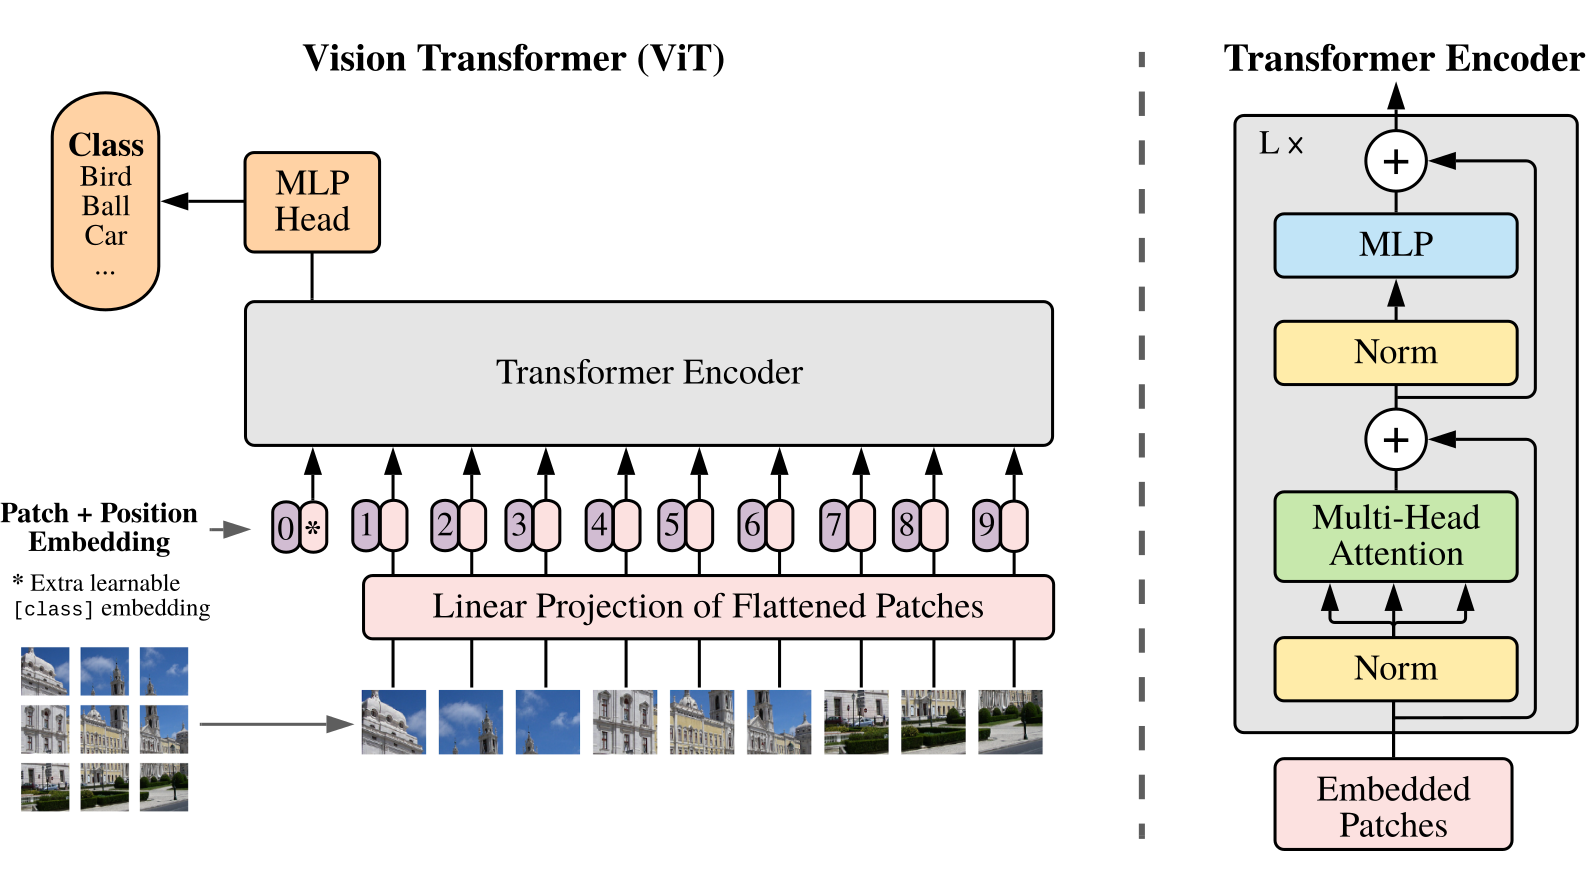
\includegraphics[width=0.8\textwidth]{vit.png}
	\caption{The Vision Transformer splits an image into patches, embeds them,
		and feeds them into a Transformer encoder. Classification is learned
		via an MLP head following the encoder. Figure reproduced
		from~\citet{dosovitskiy2021vit}}
	\label{fig:vit}
\end{figure}


\subsection{CLIP}
\label{ssec:clip}

\citet{radford2021clip} introduced CLIP (Contrastive Language-Image
Pre-training), which uses the Info-NCE loss~\citep{oord2019infonce} to jointly
learn relationships between encodings of text captions and extracted feature
representations of associated images. The Info-NCE loss trains a multimodal
embedding space to maximise the cosine similarity of matching pairs of captions
and images, while minimising the cosine similarity of non-matching pairs in the
batch. The approach is shown in \cref{fig:clip}. A key part of this approach is
using a very large batch, so that there are many incorrect pairings to learn
from. \citet{radford2021clip} use a batch size of 32768. The text encoder is a
Transformer~\citep{vaswani2017attention}, and their best model uses a Vision
Transformer~\citep{dosovitskiy2021vit} as the image encoder.

The model enables zero-shot transfer to many downstream computer vision
classification tasks by predicting the most probable (image, text) pair when
given an image and a set of text prompts with each class embedded in the prompt
achieving performance comparable to or surpassing the previous state of the art
by finetuned models. The representations learned by the contrastive
pre-training objective have wide applicability to a range of VLM and Video
Language Models, particularly as frozen features from which to add smaller
modules on top for adapting to vision and language
tasks~\citep{alayrac2022flamingo,lin2022evl,luo2022clip4clip}. We discuss some
of these models in \cref{sec:vidlmb}, and consider the limitations and possible
expansions of the contrastive pre-training method in \cref{sec:contrastive}.

\begin{figure}[tp]
	\centering
	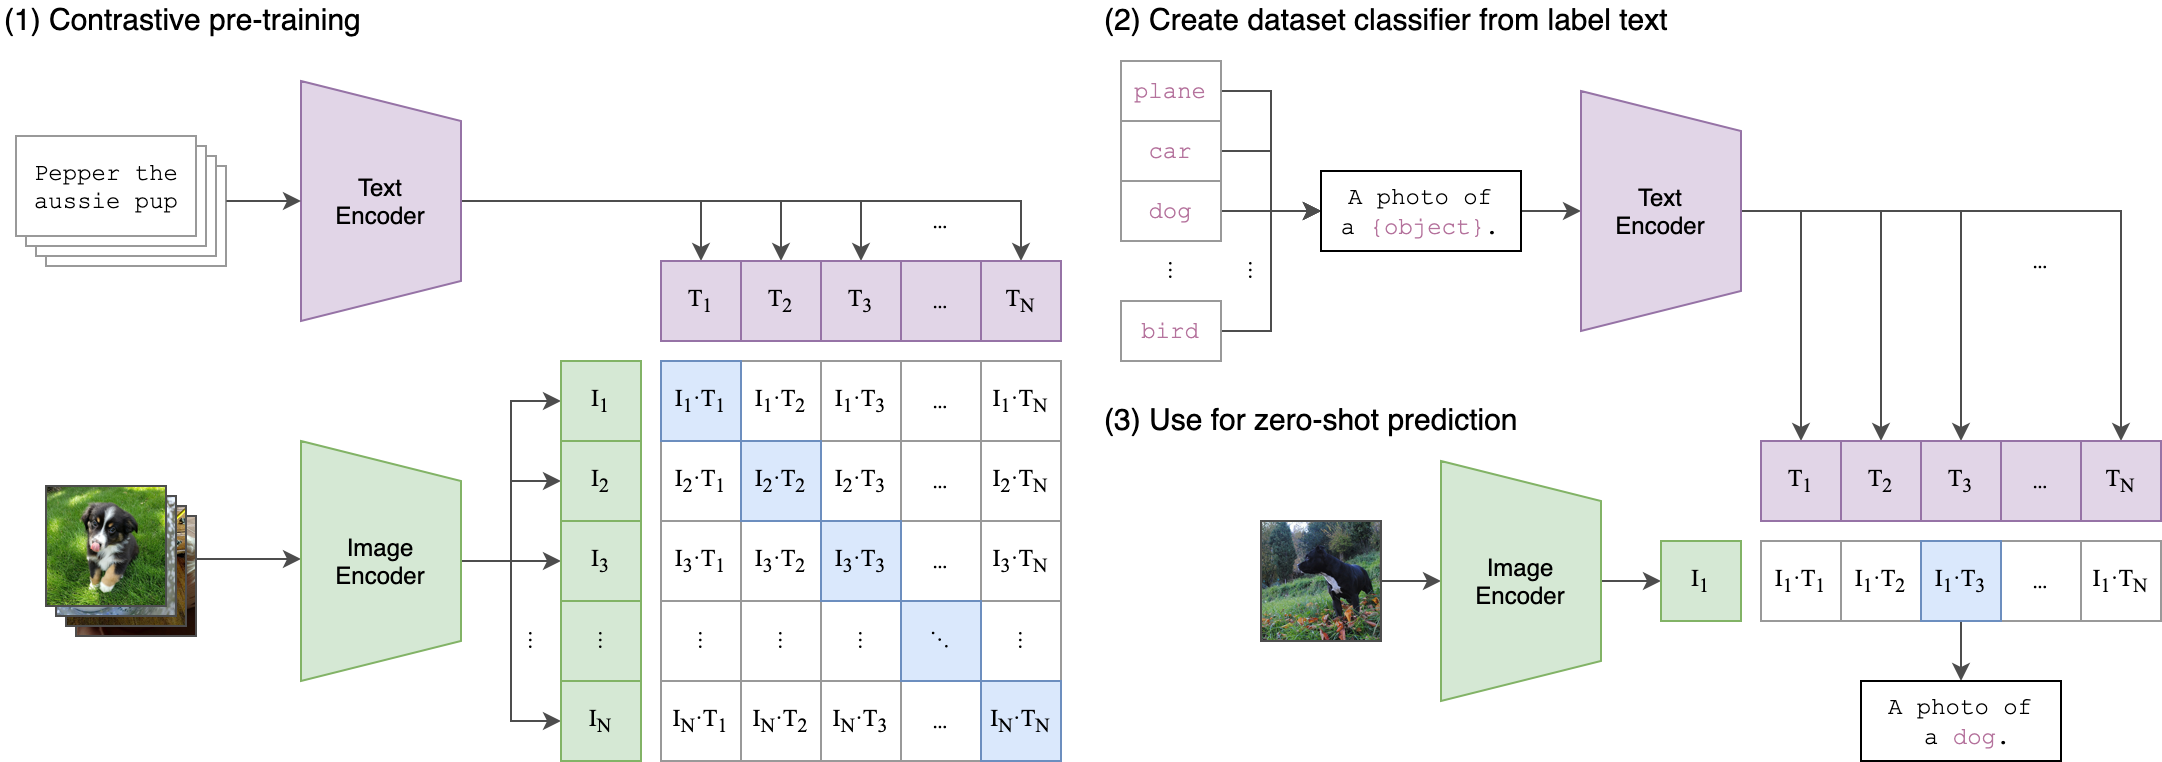
\includegraphics[width=\textwidth]{CLIP.png}
	\caption{CLIP. From~\citet{radford2021clip}}
	\label{fig:clip}
\end{figure}


\section{Vision and Language Models}
\label{sec:vlm}

One criticism of language models is that the representations learned by
training a model to predict the next word fail to learn any kind of
meaning~\citep{bender2020climbing} without reference to the real world. Models
trained in this way learn connections between surface forms, but no grounded
meaning between the form and intent portrayed through the form. A way to create
grounded representations may be to combine the two modalities of language and
vision through multimodal embeddings. A key challenge in recent years has been
to find suitable methods for creating these shared representations.

Following the strong performance in NLP of BERT~\citep{devlin2019bert},
\citet{li2019visualbert} extend BERT to include visual features extracted from a
CNN as well as text tokens as input to a Transformer encoder, implicitly
discovering a joint representation between the two modalities. The authors use
the self-attention mechanism to align elements of the input text and regions in
the input image, and pre-train on two visually-grounded language model
objectives. The authors finetune and evaluate on a range of vision and language
applications, including visual question answering (see below).

%\cite{lu2019vilbert}

Other approaches take frozen encodings of image, text, or both, and learn a
shared embedding space on top of this (e.g. BLIP-2 \citep{li2023blip2})

%Many approaches, joint training with concatenated image and text features into
%BERT (VisualBERT), learning both image and text features concurrently.


\subsection{Visual Question Answering}
\label{ssec:vqa}

Visual question answering is the task of answering questions given text and an
image. There are a wide range of datasets (name some). A challenge in creating
datasets is to ensure that there are few statistical biases or shortcuts in the
answer distribution that a model can exploit without a true understanding of
the scene. For example, models trained on the VQA dataset~\citep{antol2015vqa}
were found to make predictions based on overly strong language priors without
considering the associated image~\citep{zhang2016yin} (a green banana may trip
up a model) and failed to show complete question understanding, settling on an
answer before receiving the full question ~\citep{agrawal2016analyzing}.
Questions generally required little reasoning or compositionality, with many
answers achievable solely by object recognition~\citep{hudson2019gqa}. The GQA
dataset~\citep{hudson2019gqa} is one dataset that aims to limit these issues
by generating questions with linguistic diversity and a large vocabulary, and
balancing the answer distribution through sampling. 

Visual question answering has also been extended to question answering over
videos. On top of scene understanding, video question answering requires event
understanding to understand causal and temporal relationships within the
context of the video. A particular challenge in developing models for this task
is combining and aligning the modalities of text, vision, and audio as well.
Numerous datasets have been proposed for this task,
e.g.~\citet{xu2016msr-vtt,wu2021star,xiao2021nextqa,lei2020tvqaplus}. We discuss
two, STAR~\citep{wu2021star} and NExT-QA~\citep{xiao2021nextqa}, in
\cref{chap:dataset}.


\section{Video Language Models}
\label{sec:vidlma}

%Models which solve video tasks. How to choose frames, methods for learning
%temporal aspect, modeling sequences of images
Much as the task of visual question answering has been extended to the domain
of video, so too have models been created for video language tasks. Video
language models are models used to solve problems related to video
understanding tasks. This introduces the added complexity of temporal modeling
to understand relationships between successive frames in the video, as well as
the possibility of modeling audio where the data allows it. There are two main
ways of solving these tasks. The first is to use pretrained vision and language
models we saw previously to the new domain without any specific training or
finetuning on a video dataset.  Alternatively, we can train on a video dataset,
either from scratch, or finetuning from a pretrained vision and language model.
This section explores both methods.

\subsection{Adapted from Vision and Language Models}
\label{ssec:adaptvlm}

Pre-trained generative language models have shown strong capabilities for
in-context learning~\citep{brown2020gpt3}. In-context learning provides a number
of examples of a task (for few-shot learning -- zero-shot learning provides only
a task description) as the start of a prompt to a language model, where a
typical example contains the context of the task and its desired completion.
The language model must then provide the correct completion when presented with
just the example context. This idea, and extensions, have been shown to be
effective for a wide range of tasks, particularly those which require advanced
reasoning~\citep{wei2022cot,kojima2022step}.

By providing generative language models with access to image features in its
prompt, it is possible to leverage pre-trained language models for video tasks.
\citet{wang2022vidil} use a vision and language model to label objects, events
and attributes, as well as captions, for each sampled frame in a video. These
features are then composed in a template for few-shot learning of video tasks.
Temporal relationships between frames are modeled in the template using textual
indicators (`first', `then', `finally'). Crucially, no finetuning of language
or vision and language models is performed, so high quality pretrained models
can be plugged in and changed easily. This process is highly dependent on
strong visual feature extraction, meaning that key low-level features may be
lost if the vision models are not strong enough. Concurrent work
by~\citet{zeng2023socratic} finds that using stronger vision and language
models correlates with better performance when combining VLMs and LMs in a
zero-shot manner for egocentric perception. Finally, the added latency costs of
having separate models for visual tokenisation, frame captioning, and language
generation may make the overall system inadequate for practical use.

\citet{portilloquintero2021clipvidret} use CLIP features with an aggregation
function across frames to adapt to the video domain for retrieval tasks. The best
aggregation function tested was to simply average frame-level features, which
beat previous best recall@1 scores on the MSR-VTT~\citep{xu2016msr-vtt} dataset.
The authors found that using a single frame from around one second in to the
video as the aggregation function gives significantly worse recall performance
than other aggregation functions which take into account multiple frames.

By contrast, \citet{huang2018videotemporal} found that temporal understanding
plays just a small role in multiple video datasets. On two action recognition
datasets, the impact of motion accounts for just 6 percentage points of 79\%
accuracy on UCF101~\citep{soomro2012ucf101}, and 5 points of 47\% accuracy on
Kinetics~\citep{carreira2018kinetics600}, and 40\% and 35\% of classes do not
require any temporal understanding for the two datasets respectively.
\citet{buch2022revisiting} extend this finding for video language tasks, with
single frame understanding performing strongly compared to state of the art
models, ``even in settings intended for complex multi-frame event
understanding''. The key distinction between these works
and~\citet{portilloquintero2021clipvidret} is that the model selects a highly
informative frame based on its task. \citet{buch2022revisiting} propose that
their design, the atemporal probe (ATP), should be used to design better
datasets that better test efficacy of a benchmark for causal and temporal
understanding. They find a subset of NExT-QA~\citep{xiao2021nextqa} questions
that ``truly necessitate video-level understanding compared with the original
dataset''. We test on both NExT-QA and this subset, denoted
ATP\textsubscript{hard}, in our experiments.

%Either train with explicit temporal tokens (e.g.~\citet{lin2022evl} with temporal convolution and cross-frame attention, \citet{lei2021clipbert} with temporal fusion and sequential frames and word embeddings) or use language to steer temporal modality \citep{wang2022vidil,zeng2023socratic}.


%\citet{zeng2023socratic} -- Similar idea to VidIL, but zero-shot composition


\subsection{Training on Videos}
\label{ssec:vidtrain}

%Models which take into account temporal nature and train/finetune on video datasets

Since one of the questions we are interested in is how contrastive training
affects the temporal reasoning ability of video language models, this section
mainly explores models trained with a contrastive objective. We note, however,
that other models~\citep{lei2021clipbert} (and others!!) have achieved
comparable downstream performance when trained with other objectives (masked
language modeling, image-text matching, cross-modal attention).

The obvious approach for training video models is to train on videos.
\citet{luo2022clip4clip} extend image and language models to video retrieval in
a simple way by mapping sequences of image representations learned from CLIP
into a fixed video representation, and computing similarity between the CLIP
text encoding and the learned video encoding. They find that training on a
medium-sized video dataset starting from the CLIP encodings improves zero-shot
and finetuning results on multiple downstream datasets, and that attempts to
model the temporal dependency between frames (using 3D linear projections for
video features, and using similarity measurements that model sequentiality for
the video and text similarity measure) from the base CLIP model trained only on
image and text pairs do not produce better results on video tasks.

\citet{bain2021frozen} train separate visual encoder for image and video and text encoder for captions

\cite{xu2021videoclip}


%\citet{lin2022evl} -- train video recognition models from frozen CLIP features
\citet{lei2021clipbert} -- temporal fusion and sequential frames and word embeddings

\citet{alayrac2022flamingo} -- train on combination of image-text, video-text pairs datasets. Vision encoder is CLIP. Temporal embeddings are combined with visual features and processed via a resampling module, allowing for a variable number of frames to produce a fixed size visual output, which is advantageous for longer videos.

\section{Temporal Reasoning}
\label{sec:tempreason}


\noindent\textbf{In Video.}\hspace{0.2cm}
Most computer vision has studied how to model concepts and relationships
between them in the world, e.g. through object detection and segmentation in
images. To go one step further into the video domain, we need to study how to
model event knowledge. That is, how do we model recurring and meaningful
patterns and sequences of behaviour? A model must understand activities and
their components, as well as the temporal ordering of these activities to find
causal dynamics between them~\citep{elman2019event}. New datasets and models
have been proposed in recent years that aim to find computational models
capable of this event knowledge through temporal reasoning. 

As discussed in~\cref{ssec:adaptvlm}, some models can still perform well on
video datasets with just a single frame given to the model. This suggests a
requirement for more challenging datasets and tasks to learn temporal ordering
of events. \citet{grauman2022ego4d} create Ego4D, a dataset of over 3000 hours
of egocentric (first-person) video, with several associated tasks requiring
understanding of how objects change state over time, remembering temporal
windows for objects appearing in scenes, and prediction of future actions in
videos, requiring causal understanding of actions and events. For example, a
cooking video may predict the subsequent steps to making a pizza when presented
with the first steps of rolling and kneading dough. The authors identify
normalised pointwise mutual information as a means to inform the temporal
structure of sequences of actions over time, with certain action sequences
favoured over others. Learning this structure of action pairs is key to a
model's performance on these tasks.\\

\noindent\textbf{In Language.}\hspace{0.2cm}
There is a long history of studying temporal expressions in linguistics.
~\citet{moens1988temporal} claim that \textit{when}-clauses ``establish a
temporal focus'' between two events, contingent on e.g. a causal link, as in
the unnatural use of \textit{when} in ``*When my car broke down, the sun set.''
Any representation looking to model temporal descriptions must therefore, for
\textit{when}-clauses and similar phenomena, model contingency, rather than
just temporality.

\citet{allen1983interval} suggests a model of temporal reasoning based on
intervals and relations among them. Given two events, the temporal relations
between them can be expressed in many ways based on the time intervals of the
events occurring. We explore the use of this temporal representation further
in~\cref{sec:data}. \citet{zhou2021tracie} propose a dataset for natural
language inference of temporal relations for before and after relations. They
find that current models struggled to predict temporal relationships between
explicit and implicit events, and that a neuro-symbolic method improved 
reasoning ability by estimating event durations to infer implicit end times.\\

%Traditional methods
%\cite{bruce1972temporalqa}
%\cite{pustejovsky2003timeml}

%Pre-trained LLMs struggle on temporal reasoning, need finetuning.~\citet{vashishtha2020temporal}

\noindent\textbf{Probing video datasets.}\hspace{0.2cm}
\citet{sevilla-lara2021temporal} create a perceptual test to discover action
classes in videos that require temporal information to identify. The authors
shuffle frames in time from action classification datasets, and present human
annotators with the shuffled or control videos, where there is no shuffling.
Action classes are then identified by the largest average performance
degradation of action classification between the two groups. They train video
models on a temporal and static dataset, the 50 classes where human accuracy
decreases most and least respectively, and find that training on the temporal
dataset produces features that are more sensitive to temporal ordering, and
therefore are stronger temporal features.
We extend this finding and explore the performance of various models with
frames shuffled on video question answering datasets in \cref{chap:probe}, and
develop a novel method for training video language models on a temporal-aware
dataset in \cref{chap:setup}.

%\section{Video Question Answering}
%\label{sec:vidqa}
%
%\subsection{STAR Dataset}
%\label{ssec:star}
%
%We primarily focus on this due to its focus on sequential questions that evaluate model performance on temporal reasoning
%
%\subsection{Merlot Reserve}
%\label{ssec:mreserve}
%
%We examine a specific video language model, Merlot Reserve \citep{zellers2022mreserve}, that performs strongly on STAR.

%! TeX root = ../charles/en/thesis.tex
\chapter{Related Work}
\label{chap:rel}

This chapter looks at previous work on probing \acrlongpl{vlm},
and techniques for improving reasoning in various directions in \acrlong{vlm}s. We use
and extend the approaches explored to try and improve the temporal reasoning
abilities of \acrshortpl{vidlm}.

%\section{Video Language Models}
%\label{sec:vidlmb}
%
%CLIP-based \citep{radford2021clip} with no video data, 
%Contrastive with video data, Merlot Reserve~\cite{zellers2022mreserve}, VideoCLIP~\cite{xu2021videoclip}, \cite{luo2022clip4clip}
%Masked VLM: VideoBERT \citep{sun2019videobert}, VLM \citep{xu2021vlm}
%Separate frozen image/video approaches with finetuning/adapters: Flamingo \citep{alayrac2022flamingo}
%Separate frozen image/video approaches with prompt engineering: \citep{wang2022vidil, zeng2023socratic}


\section{Contrastive Training in \acrshortpl{vlm}}
\label{sec:contrastive}

Some previous studies have looked at the effect of contrastive pre-training in
vision and language models, and introduce the idea of post-pretraining VLMs
with hard negatives~\citep{yuksekgonul2023when, momeni2023verbs,
bagad2023testoftime}. Post-pretraining is a continuation of self-supervised
pre-training on a smaller dataset with desired properties that aid the learning
process of the model, mitigating the cost of expensive general pre-training
while allowing for specialisation of a model. This can be used for, e.g.
transferring \acrshortpl{vlm} to the video domain with a small video dataset,
as in~\citet{luo2022clip4clip}, discussed in \cref{ssec:vidtrain}. Or, as we
discuss in this chapter, instilling better understanding of concepts and
relationships with targeted hard negatives in a contrastive objective.
\citet{yuksekgonul2023when} explore compositional relationships in
\acrlongpl{vlm} by testing existing \acrshortpl{vlm} on a dataset with
perturbations exploring attributive understanding of adjectives to nouns,
relational understanding for prepositions and verbs, and sensitivity to word
order in image captions. When presented with an original caption and its
transformation(s), models must predict which caption is more likely. The
authors find that most models are deficient in relational understanding tasks
(e.g. choosing between `the horse is eating the grass' and `the grass is eating
the horse'), but are better at attribution of properties to objects, as in `the
paved road and the white house' vs 'the white road and the paved house'. Models
also performed close to chance on the word order sensitivity test, where
multiple extra captions were created with shuffled nouns/adjectives, shuffled
trigrams, and shuffled words within each trigram, indicating the
\acrshortpl{vlm} behave like bags-of-words.

The authors claim that this may be down to the contrastive pre-training
objective in \acrshortpl{vlm} such as \acrshort{clip}~\citep{radford2021clip},
where the retrieval nature of the objective leads to a bias towards object
recognition without considering compositionality, and that in datasets without
carefully constructed caption alternatives, order information is not required
to solve the objective. An incentive, in the form of additional hard negatives
in both alternative images and generated targeted captions, is therefore
proposed~(\cref{fig:bow_hard_negs}), which improves performance on the testing
benchmarks for attribution (62\% to 71\%), relation (63\% to 81\%), and order
(46\% to 86\% and 59\% to 91\%) substantially, while not degrading performance
in other downstream tasks.

\begin{figure}[t]
	\centering
	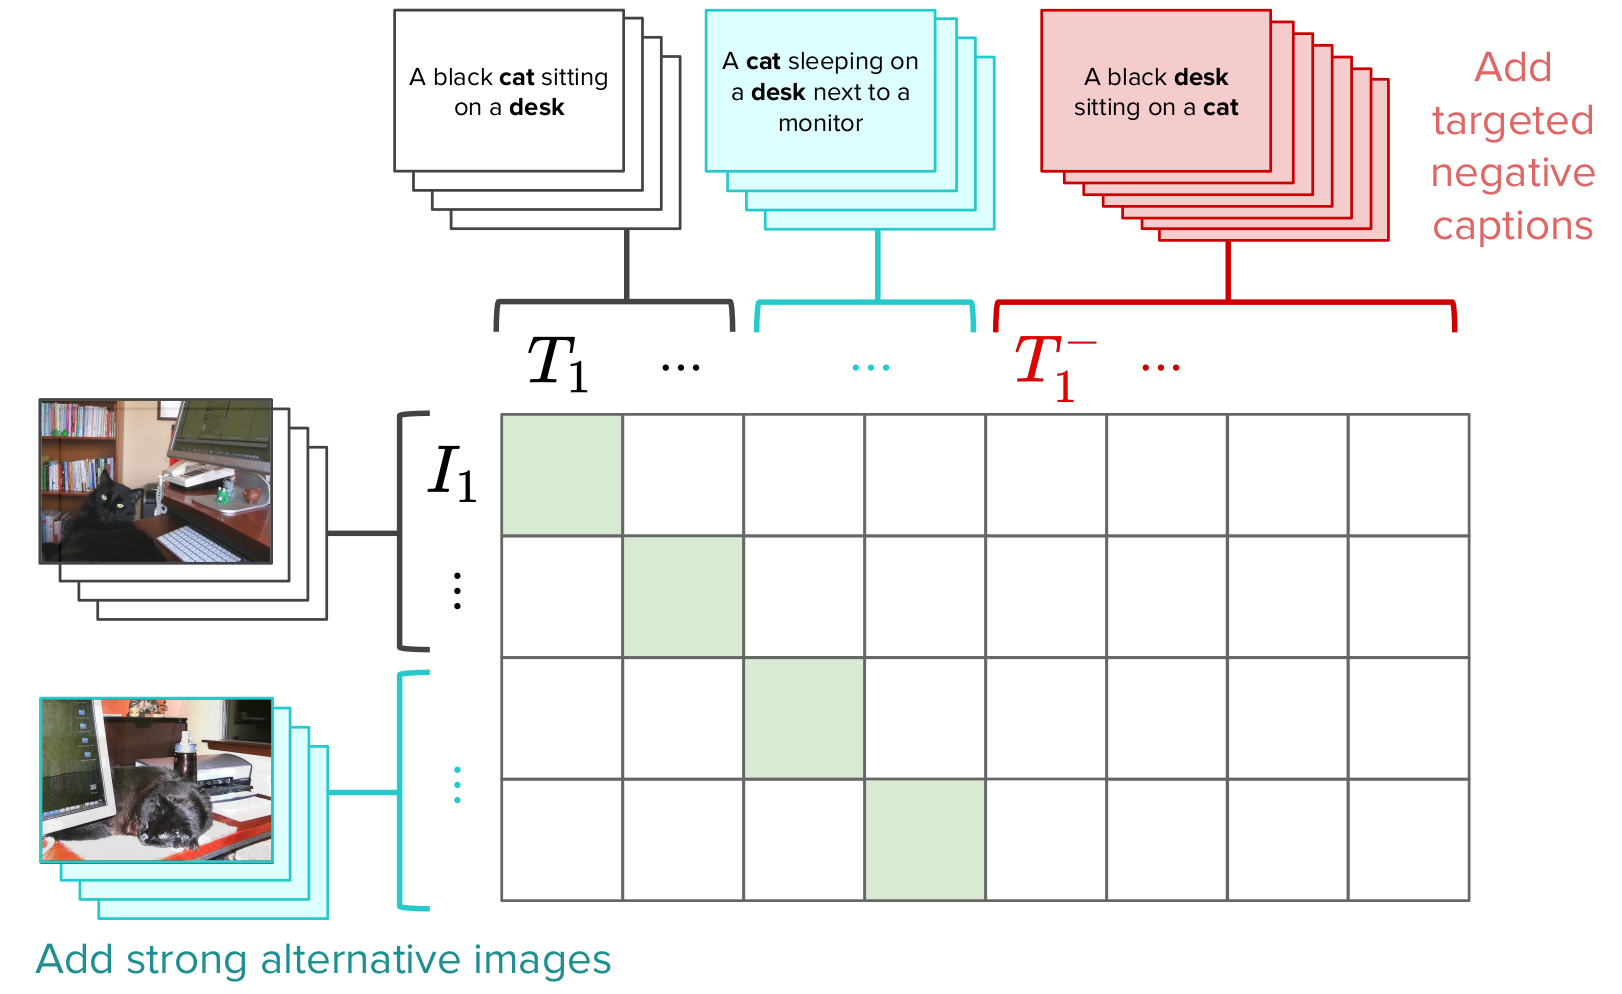
\includegraphics[width=0.8\textwidth]{bow_hard_negs.png}
	\caption{Hard negatives for contrastive learning, with generated negative
	captions and retrieved alternative images. Captions are generated by
	swapping various linguistic features, while images are sampled from 
	k-nearest neighbours. From~\citet{yuksekgonul2023when}.}
	\label{fig:bow_hard_negs}
\end{figure}


\section{Understanding in Video Language Models}
\label{sec:understandvidlm}

Here we discuss two papers that look at improving understanding in
\acrfullpl{vidlm} by extending the contrastive objectives with hard negatives
for verb understanding~\cite{momeni2023verbs}, and in before/after
relations~\cite{bagad2023testoftime}. 

\subsection{Verbs in Action}
\label{ssec:verbs}
\citet{momeni2023verbs} look at \acrshortpl{vidlm} trained with a contrastive
loss function, and find similar issues with verb understanding to those
identified by~\cite{yuksekgonul2023when}. They propose to generate hard
negatives with modified verb phrases using pre-trained \acrfullpl{llm}, as well
as introducing an additional verb phrase alignment loss which contrastively
compare a verb phrase from the positive caption to other verb phrases in the
batch to provide an additional focus on verbs to the model
(see~\cref{fig:vfc}). As in~\cite{yuksekgonul2023when}, models trained with
targeted alternatives improve performance for datasets that require
understanding of the targeted domain in both zero-shot and finetuning setups. 

\begin{figure}[t]
	\centering
	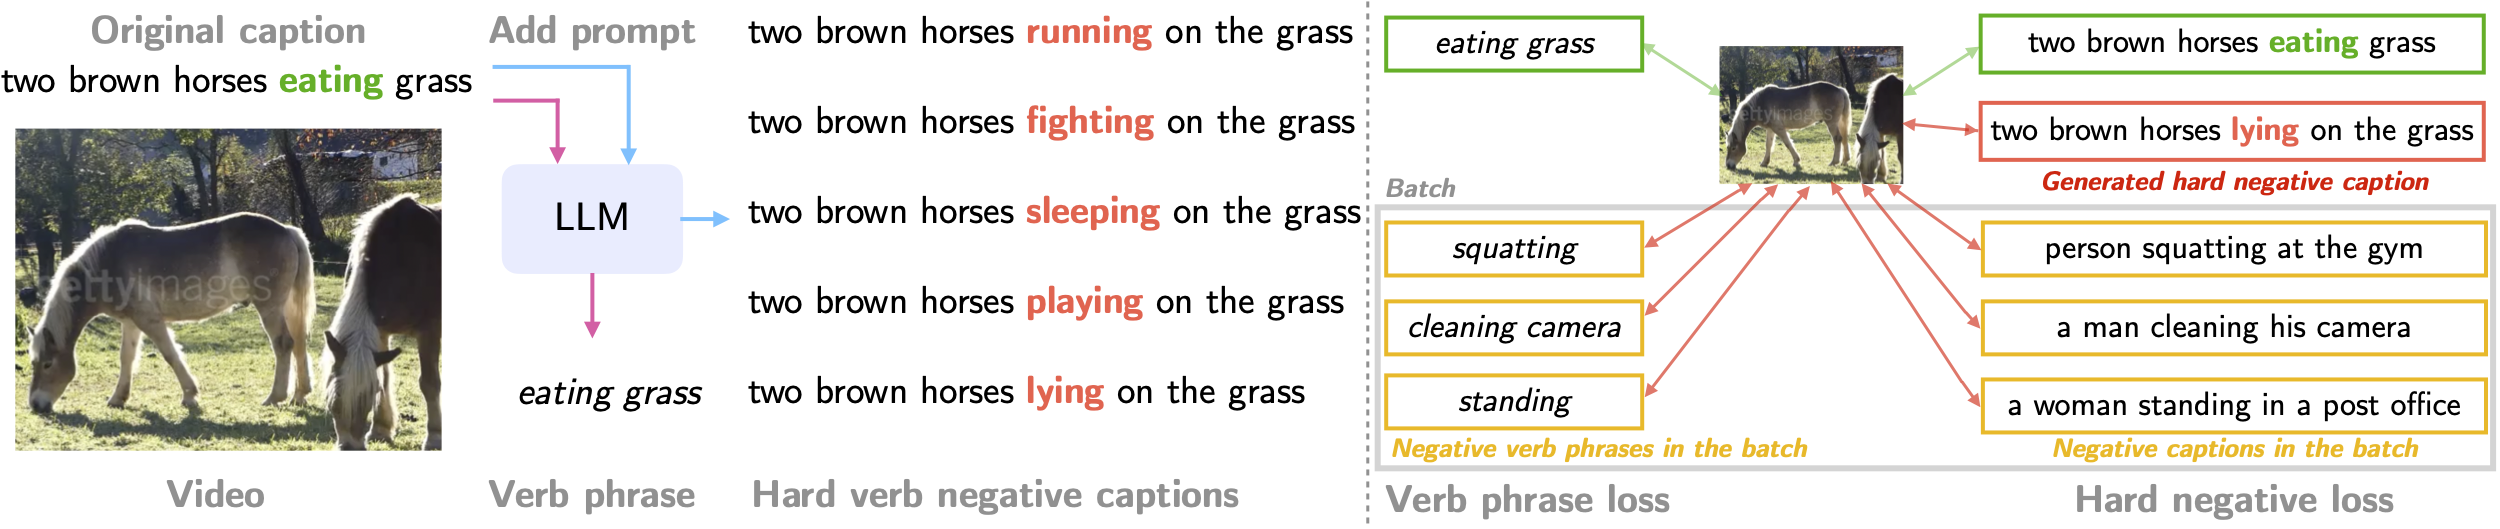
\includegraphics[width=\textwidth]{vfc.png}
	\caption{Verb-Focused Contrastive learning. Generated negative captions are
	added as hard negatives to the contrastive loss objective.
	From~\cite{momeni2023verbs}.}
	\label{fig:vfc}
\end{figure}


%InfoNCE loss, work in similar training styles for different domains
%\citep{momeni2023verbs, yuksekgonul2023when}.

\subsection{Test of Time}
\label{ssec:testoftime}
The most similar paper to our work is~\cite{bagad2023testoftime}. The authors
look at before/after relations in videos by using a synthetic dataset to
probe existing models. They construct videos containing pairs of events such
as ``a red circle appears before a yellow circle'', and create distractor
annotations by reversing the order of events but keeping the temporal relation
the same. On this time-order probing task, they find that existing models
perform no better than chance for the task of associating the correct
annotation to the video. They describe a post-pretraining strategy, Temporal
Adaptation by Consistency of Time-order (TACT), for improving the understanding
of before/after relations in \acrshortpl{vidlm}, where non-overlapping video
clips are stitched together and paired with a text description that consists of
the clip captions and a temporal relation, either before or after, to match the
order of the combined video clip (see~\cref{fig:tact}). A reversal function is
then applied to create hard negative examples by reversing the order of text
captions or video clips, which are included as negatives in the contrastive
post-pretraining objective.

\begin{figure}[t]
	\centering
	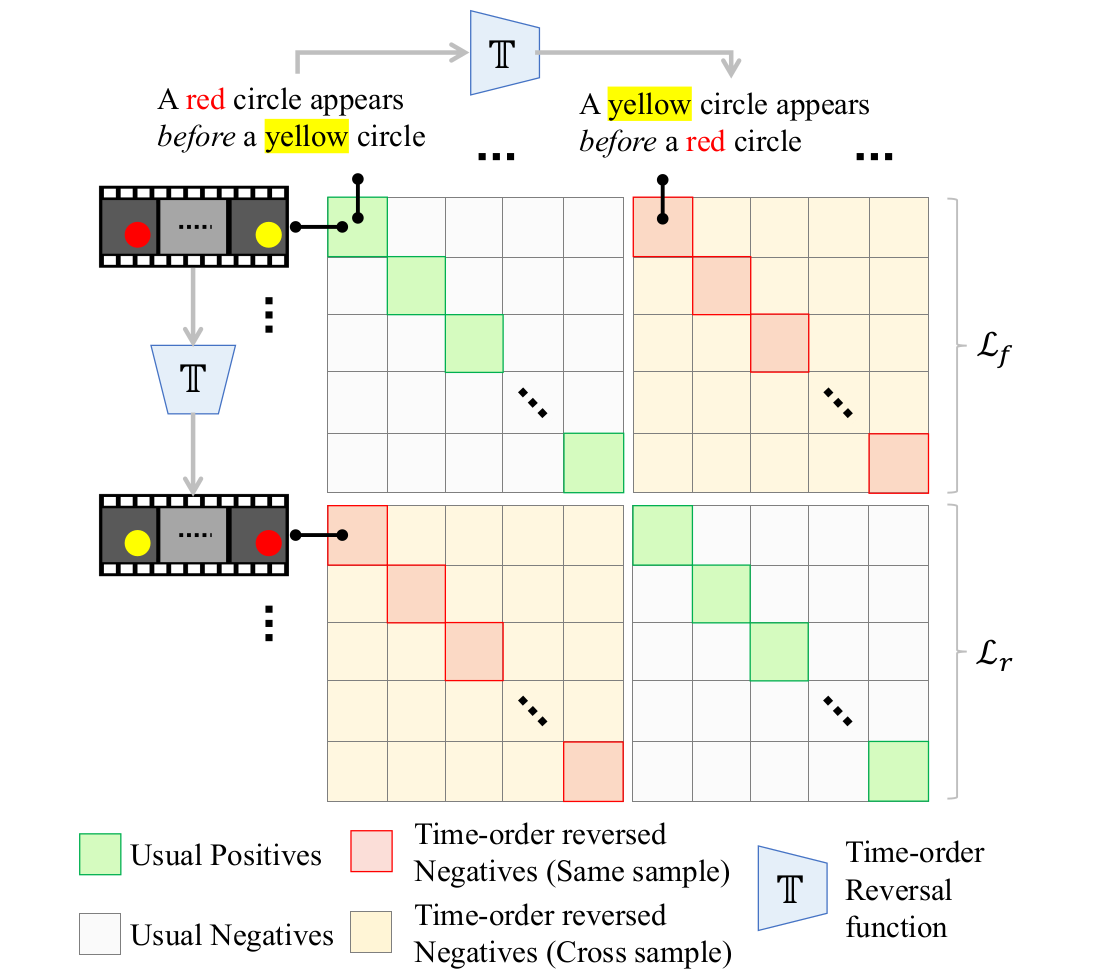
\includegraphics[width=0.8\textwidth]{tact.png}
	\caption{Temporal Adaptation by Consistency of Time-order. Extra negatives
	are included by reversing time-order in annotations and videos. Figure
	from~\citet{bagad2023testoftime}.}
	\label{fig:tact}
\end{figure}

They find that this approach improves performance on the time-order probing
task, with models much more likely to match the correct caption to the stitched
video clips. On downstream tasks, they find a mixed result. On video retrieval
tasks, on which claim existing datasets have more of a bias towards spatial
understanding than temporal reasoning
(see~\cref{ssec:adaptvlm};~\citet{buch2022revisiting,lei2023revealing,luo2022clip4clip}),
the model performs slightly worse in general than without using the TACT
approach. On \acrlong{vidqa}, with temporally challenging datasets, there are
generally slight improvements. For example on the NExT-QA
ATP\textsubscript{hard} subset, the TACT model trained on clips from
TEMPO~\citep{hendricks2018tempo} achieves a zero-shot accuracy of 27.6,
compared to 25.0 on the baseline model.  However, on clips from the Charades
dataset~\citep{sigurdsson2016charades} the TACT performance is worse than the
Charades baseline model (25.2 vs 26.0). They find that the TACT model generally
improves performance on action recognition benchmark subsets which have been
identified as requiring temporal information. 

In comparison to~\cite{bagad2023testoftime}, we explore different ways of
probing temporal understanding, use a wider range of temporal relations with
full videos, and aim to gain stronger relationship between frame and action
with the contrastive span objective. We fully compare our approaches and
results in~\cref{sec:tactcompare}.


\chapter*{Conclusion}
\addcontentsline{toc}{chapter}{Conclusion}
%! TeX root = ../charles/en/thesis.tex
\label{chap:conclusion}

In this thesis, we investigated the ability of \acrfullpl{vlm} to reason across
time. We found that current models, trained with a contrastive learning
objective, do not use temporal indicators, even for questions that ought to
require them. When predicting whether one action happens before or after
another, models perform at chance at best. Following previous work, we
attempted to instill a sense of temporal reasoning into one specific model,
Merlot Reserve. We use hard negatives focussed on temporal expressions to make
models more sensitive to temporal cues, with the expectation that performance
on tasks that require temporal information would improve, and that models would
become more robust to misleading temporal information, such as the examples
shown in \cref{chap:probe}.

We proposed a new dataset based on Charades~\citep{sigurdsson2016charades} for
the Merlot Reserve model~\citep{zellers2022mreserve}. This dataset added
focussed hard negatives to segments which include a temporal expression.
Training on this dataset, with hard negatives included as additions to the
contrastive loss function, we found that our model improved on zero-shot
downstream \acrshort{vidqa} tasks, but did not show clear signs of improvement
in our probing tests. We did find some qualitative suggestions of more model
uncertainty, however.

%we found that our model was able to perform better
%at identifying order in video when asked to identify whether one event happens
%before or after another, although this did not translate to overall better
%performance on benchmarks. There were also mixed results on other probing
%tests: swapping the question asked; and shuffling the order of frames provided
%to the model. 

This may be down to the multiple choice nature of the datasets,
which often do not provide distractor options that are incorrect in the sense
of time. Future work may consider this as an added dimension to challenge
models in when considering multiple-choice video question answering. Open-ended
\acrshort{vidqa} was not considered here, since the models we evaluate are not
able to generate text, but it may be an interesting study to compare our
probing methods with the generated answers given for open-ended
\acrshort{vidqa} datasets.

Finally, there are technical changes and optimisations that could be made. As
noted in~\cref{ssec:clip}, contrastive learning often requires large batches to
work effectively. The largest batch size we were able to train with was 8,
which is at least an order of magnitude away from batch sizes considered by
previous work. We also acknowledged that the frame selection process at
inference time could be improved, and suggested an approach for selecting more
informative frames from a video. 





%%% Bibliography
%%% Bibliography (literature used as a source)
%%%
%%% We employ bibTeX to construct the bibliography. It processes
%%% citations in the text (e.g., the \cite{...} macro) and looks up
%%% relevant entries in the bibliography.bib file.
%%%
%%% The \bibliographystyle command selects, which style will be used
%%% for references from the text. The argument in curly brackets is
%%% the name of the corresponding style file (*.bst). Both styles
%%% mentioned in this template are included in LaTeX distributions.

\bibliographystyle{plainnat}    %% Author (year)
% \bibliographystyle{unsrt}     %% [number]

\renewcommand{\bibname}{Bibliography}

%%% Generate the bibliography. Beware that if you cited no works,
%%% the empty list will be omitted completely.

\bibliography{bibliography}

%%% If case you prefer to write the bibliography manually (without bibTeX),
%%% you can use the following. Please follow the ISO 690 standard and
%%% citation conventions of your field of research.

% \begin{thebibliography}{99}
%
% \bibitem{lamport94}
%   {\sc Lamport,} Leslie.
%   \emph{\LaTeX: A Document Preparation System}.
%   2nd edition.
%   Massachusetts: Addison Wesley, 1994.
%   ISBN 0-201-52983-1.
%
% \end{thebibliography}


%%% Figures used in the thesis (consider if this is needed)
\listoffigures

%%% Tables used in the thesis (consider if this is needed)
%%% In mathematical theses, it could be better to move the list of tables to the beginning of the thesis.
\listoftables

%%% Abbreviations used in the thesis, if any, including their explanation
%%% In mathematical theses, it could be better to move the list of abbreviations to the beginning of the thesis.
\chapwithtoc{List of Abbreviations}

%%% Attachments to the master thesis, if any. Each attachment must be
%%% referred to at least once from the text of the thesis. Attachments
%%% are numbered.
%%%
%%% The printed version should preferably contain attachments, which can be
%%% read (additional tables and charts, supplementary text, examples of
%%% program output, etc.). The electronic version is more suited for attachments
%%% which will likely be used in an electronic form rather than read (program
%%% source code, data files, interactive charts, etc.). Electronic attachments
%%% should be uploaded to SIS and optionally also included in the thesis on a~CD/DVD.
%%% Allowed file formats are specified in provision of the rector no. 72/2017.
\appendix
\chapter{Attachments}

\section{First Attachment}


\openright
\end{document}
